\EnglishSourceFrame{GELFAND-P001395}{unlabelled}
\underline{19.10.87.}\quad \underline{Gelfand seminar.}

\underline{I. M. Gelfand}\quad
\underline{Calculating sums of $k$th powers and other sums}

\EnglishUnclear{GELFAND-P001395}{speaker-parenthesis}{(following a recent thought) / (following an unclear thought)}

\begin{equation*}
F'(x)=f(x)\qquad f(x)=x^k;\qquad F(x)=\frac{x^{k+1}}{k+1}
\end{equation*}
\begin{align*}
F(2)-F(1)&=\frac{f(1)}{1!}+\frac{f'(1)}{2!}+\frac{f''(1)}{3!}+\ldots\\
F(3)-F(2)&=\frac{f(2)}{1!}+\frac{f'(2)}{2!}+\frac{f''(2)}{3!}+\ldots\\[8pt]
F(n+1)-F(n)&=f(n)+\frac{f'(n)}{2!}+\frac{f''(n)}{3!}+\ldots
\end{align*}
\rule{9cm}{0.3pt}
\begin{equation*}
F(n+1)-F(1)=S_0+\frac{S_1}{2!}+\frac{S_2}{3!}+\ldots
\end{equation*}
Similarly,
\begin{align*}
f(n+1)-f(1)&=S_1+\frac{S_2}{2!}+\ldots\\
f'(n+1)-f'(1)&=S_2+\frac{S_3}{2!}+\ldots\\
\ldots\qquad&\ldots\\
f^{(p)}(n+1)-f^{(p)}(1)&=\ldots\quad
\EnglishUnclear{GELFAND-P001395}{system-last-index}{S_p}+\ldots
\end{align*}

[To the right of the system:]
Here
\begin{align*}
S_0&=f(1)+f(2)+\ldots+f(n)\\
S_1&=f'(1)+f'(2)+\ldots+f'(n)\\
&\ldots\\
S_k&=f^{(k)}(1)+f^{(k)}(2)+\ldots+f^{(k)}(n)
\end{align*}

Hence
[to the left of the determinant, crossed out:
\EnglishUnclear{GELFAND-P001395}{determinant-cancellation}{det / illegible}]
\begin{equation*}
S_0=\frac{
\begin{vmatrix}
F(n+1)-F(1)&\dfrac{1}{2!}&\dfrac{1}{3!}&\ldots\\
f(n+1)-f(1)&1&\dfrac{1}{2!}&\\
f'(n+1)-f'(1)&0&1&\\
\ldots&0&0&
\end{vmatrix}}{1}
\end{equation*}

Expand along the first column:
\begin{equation*}
S_0=A_0\bigl(F(n+1)-F(1)\bigr)
+A_1\bigl(f(n+1)-f(1)\bigr)+\ldots
\end{equation*}
The coefficients are universal---valid for $\forall$ functions!!

Substitute $f(x)=e^{tx}$.

Banded determinants arise!

[Crossed out:
\EnglishUnclear{GELFAND-P001395}{exponential-cancellation}{$S_0=A_0$ / illegible}]
\begin{equation*}
\EnglishUnclear{GELFAND-P001395}{exponential-fraction}{\frac{\dfrac{1}{n+1}e^{t(n+1)}-e}{e^t-1}}
\end{equation*}
Expand [crossed out:
\EnglishUnclear{GELFAND-P001395}{series-cancellation}{series / illegible}]
in $t$\quad $\Longrightarrow$ \underline{Bernoulli numbers}.

\underline{Problem.} The symmetric group $S_n$
\EnglishUnclear{GELFAND-P001395}{symmetric-group-predicate}{is generated / is defined}
[inserted above the line: ``(\EnglishUnclear{GELFAND-P001395}{group-generator-abbreviation}{obrts. / obr. [unexpanded source abbreviations]} $s_1,\ldots,s_{n-1}$)'']
by the relations
\begin{equation*}
s_i^2=1,\qquad s_i s_j=s_j s_i\quad\text{for }|i-j|\ge2,
\qquad (s_i s_{i+1})^3=1
\end{equation*}
Consider a parabolic subgroup:
\begin{equation*}
G=\Sigma_n,\qquad H=\Sigma_k\times\Sigma_{n-k},\qquad G\supset H
\end{equation*}
\begin{equation*}
\mathcal A=\mathbb C[G]=
\left\{\sum_{g\in G}a_g g,\quad a_g\in\mathbb C\right\}
\end{equation*}


\EnglishSourceFrame{GELFAND-P001396}{23}
\begin{equation*}
\mathcal A\supset
\underset{\text{subalgebra}}{\mathcal A'}
=\{x\in A,\ xh=hx=x\text{ for every }h\in H\}
\end{equation*}

[Crossed-out sign before the heading:
\EnglishUnclear{GELFAND-P001396}{heading-cancellation}{illegible}]
\underline{Beilinson A.}\quad (continued)

\underline{Derived categories}

\begin{tikzcd}[row sep=small,column sep=small]
\mathcal A\arrow[d]&\text{--- an abelian category}\\
C(\mathcal A)\arrow[d]&\text{--- the category of complexes over }\mathcal A\\
K(\mathcal A)\arrow[d]&\text{--- the homotopy category}\\
D(\mathcal A)&\text{--- the derived category}
\end{tikzcd}

The objects of $D(\mathcal A)$ are complexes; the morphisms are equivalence classes of diagrams.

\EnglishSourceFigure{GELFAND-P001396}{roof-cancellation}{A crossed-out diagram: $X$ above on the left, $Y$ above on the right, $Z$ below between them; slanting strokes from the lower node towards the upper ones and a broad repeated zigzag cancellation are visible. The exact arrow strokes beneath the cancellation cannot be established.}

\begin{center}
\begin{minipage}[t]{.46\linewidth}\vspace{0pt}\centering
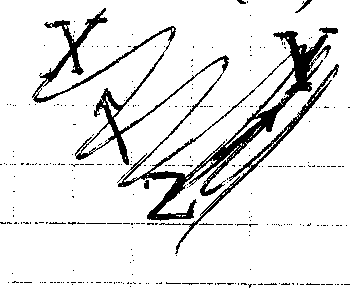
\includegraphics[width=\linewidth]{figures/gelfand-0152-p001396-roof-original-r2.png}\par\smallskip
{\footnotesize Original manuscript detail: \texttt{GELFAND-P001396}}
\end{minipage}\hfill
\begin{minipage}[t]{.50\linewidth}\vspace{0pt}\centering
{\footnotesize Partial visible-stroke recreation}\par\smallskip
% Partial visible-stroke recreation. No hidden morphism direction is supplied.
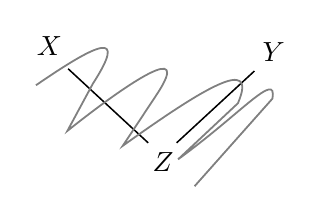
\begin{tikzpicture}[x=.95cm,y=.95cm,line width=.55pt]
\node at (0,1.25) {$X$};
\node at (3,1.18) {$Y$};
\node at (1.52,-.3) {$Z$};
\draw (.25,.95)--(1.32,-.04);
\draw (1.7,-.04)--(2.74,.92);
\draw[gray,line width=.65pt] (-.18,.73)
  .. controls (.65,1.3) and (1.05,1.48) .. (.58,.75)
  --(.24,.12) .. controls (1.12,.82) and (1.88,1.3) .. (1.45,.63)
  --(.98,-.08) .. controls (2.03,.67) and (2.8,1.15) .. (2.52,.49)
  --(1.72,-.26) .. controls (2.56,.35) and (3.05,.94) .. (2.98,.55)
  --(1.94,-.62);
\end{tikzpicture}

\end{minipage}
\end{center}
\noindent{\small\textit{The cancelled nodes are readable, but the directions beneath cancellation are not recovered. Plain connecting strokes do not assert morphisms.}}


\begin{tikzcd}[row sep=small,column sep=small]
&Z'&\\
X\arrow[ur]&&Y\arrow[ul,shorten <=8pt,shorten >=8pt]\\
&Z\arrow[ul,shorten <=8pt,shorten >=8pt]\arrow[ur]&
\end{tikzcd}
\quad (quasi-isomorphisms are shorter).

\underline{Example 1.} Let $X$ be a complex with
[crossed out: \EnglishUnclear{GELFAND-P001396}{example-cancellation}{so [unresolved source fragment] / illegible}]
$H^i(X)=0$ for $i\ne0$.
Then $X$ is canonically quasi-isomorphic to $H^0(X)$:
\begin{equation*}
X\cong H^0(X)\text{ in }D(\mathcal A)
\end{equation*}
(This is not so in the homotopy category!)

For the complex $X$, introduce the subcomplex $\tau_{\le0}(X)$ in $X$:
\begin{equation*}
\text{(1)}\qquad
\tau_{\le0}(X)^i=
\begin{cases}
X^i,&i<0\\
\ker d:X^0\to X^1,&i=0\\
0,&i>0
\end{cases}
\end{equation*}
It is easy to see that
\begin{equation*}
\text{(2)}\qquad
H^j(\tau_{\le0}(X))=
\begin{cases}
H^j(X),&j\le0\\
0,&j>0
\end{cases}
\end{equation*}
The diagram

(3)
\EnglishSourceFigure{GELFAND-P001396}{truncation-diagram}{At the bottom is $\tau_{\le0}(X)$; arrows go from it upwards to the left towards $X$ and upwards to the right towards $H^0(X)$. The right arrow has $\sim$. Beside the left arrow is a sign resembling a rotated tilde, $2$ or $\iota$; below on the left is the caption ``canonical inclusion''. To the right of the diagram is a separate short hook-shaped stroke.}

\def\GelfandCanonicalInclusionCaption{canonical\\inclusion}
\begin{center}
\begin{minipage}[t]{.46\linewidth}\vspace{0pt}\centering
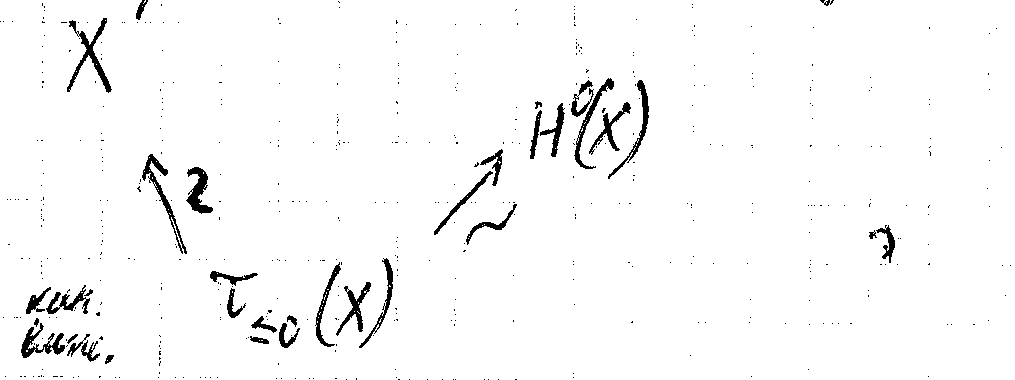
\includegraphics[width=\linewidth]{figures/gelfand-0152-p001396-truncation-original-r2.png}\par\smallskip
{\footnotesize Original manuscript detail: \texttt{GELFAND-P001396}}
\end{minipage}\hfill
\begin{minipage}[t]{.50\linewidth}\vspace{0pt}\centering
{\footnotesize Partial visible-stroke recreation}\par\smallskip
% Requires the language-local caption macro \GelfandCanonicalInclusionCaption.
% The label on the left remains a candidate list, not a selected reading.
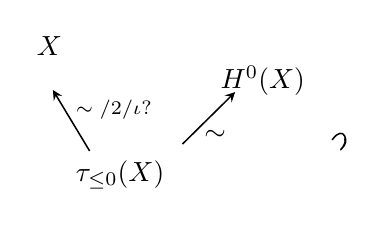
\begin{tikzpicture}[x=.88cm,y=.88cm,line width=.55pt,>=stealth]
\node at (0,1.55) {$X$};
\node at (3.08,1.05) {$H^0(X)$};
\node at (1.02,-.30) {$\tau_{\le0}(X)$};
\draw[->] (.58,.04)--(.05,.92);
\draw[->] (1.92,.14)--(2.68,.89);
\node[font=\scriptsize] at (.93,.64) {$\sim/2/\iota$?};
\node at (2.39,.26) {$\sim$};
\node[font=\scriptsize,align=center] at (-.18,-.33) {\GelfandCanonicalInclusionCaption};
% The isolated right-hand ink stroke has no assigned mathematical meaning.
\draw (4.08,.20) .. controls (4.25,.44) and (4.34,.16) .. (4.22,.08)
  .. controls (4.16,.02) and (4.30,.13) .. (4.26,.22);
\end{tikzpicture}

\end{minipage}
\end{center}
\noindent{\small\textit{The left arrow label remains tilde/2/iota candidates. Its being a quasi-isomorphism in this example does not settle the written sign. The isolated right stroke is retained without interpretation.}}


defines the required isomorphism in $D(\mathcal A)$.

[Crossed out:
\EnglishUnclear{GELFAND-P001396}{cancelled-bottom-sentence}{This same complex could have been looked at}]

\underline{Remark.} A complex $X$ with several non-$0$ groups $H^i$
is \underline{not} quasi-isomorphic (in general) to their sum, and if
[inserted above the line: ``(quasi)''] it is, then not uniquely.


\EnglishSourceFrame{GELFAND-P001397}{unlabelled}
\underline{The structure of a triangulated category}

$K(A)$ and $D(A)$ are not abelian categories.

\underline{Exercise 1.} Check that
$K(A)$ is abelian $\Longleftrightarrow\mathcal A$ is semisimple

($\mathcal A$ is semisimple $\Longleftrightarrow$
$[(\forall\text{ object})=(\text{a direct sum of irreducibles})]$).

\underline{The cone of a morphism.}

Let $f:X\longrightarrow Y$\quad be a morphism of complexes.

\begin{tikzcd}[row sep=small,column sep=large]
X^1\arrow[r,"f^1"]\arrow[dr,dashed,no head]&Y^1\\
X^0\arrow[u]\arrow[r,"f^0"]\arrow[dr,dashed,no head]&Y^0\arrow[u]\\
X^{-1}\arrow[u]\arrow[r,"f^{-1}"]&Y^{-1}\arrow[u]
\end{tikzcd}

Consider all of this as a bicomplex, i.e.
write the complex
\begin{equation*}
C(f)^i=\EnglishUnclear{GELFAND-P001397}{cone-coordinate-order}{Y^i\oplus X^{i+1}}
\end{equation*}
\begin{equation*}
d(x,y)=(-d(x),d(y)+f(x))
\end{equation*}

There is a sequence
\begin{equation*}
\text{(4)}\qquad
C(f[-1])\longrightarrow X\overset{f}{\longrightarrow}Y
\underset{g}{\longrightarrow}C(f)\longrightarrow X[1]\longrightarrow
\end{equation*}
[Above the arrow $Y\to C(f)$, crossed out:
\EnglishUnclear{GELFAND-P001397}{sequence-arrow-cancellation}{illegible};
beneath $g$: ``inclusion''.]
[Before $C(f)$, crossed out:
\EnglishUnclear{GELFAND-P001397}{sequence-object-cancellation}{$X$ / $Y$}.]
[Beneath $X[1]$: ``a shift of the grading and a change of sign of $d$''.]
\begin{equation*}
\longrightarrow Y(1)\longrightarrow
\EnglishUnclear{GELFAND-P001397}{sequence-shifted-cone}{C(f[1])\text{ / }C(f)[1]}
\longrightarrow X[2]\longrightarrow
\end{equation*}
[Between $X$ and $[2]$, crossed out:
\EnglishUnclear{GELFAND-P001397}{sequence-shift-cancellation}{( / [1] / illegible}.]

It goes into itself under a shift of three steps.
In the homotopy category it goes into itself under a shift of one step.

\begin{equation*}
\text{(5)}\qquad Y\overset{g}{\longrightarrow}C(f)\longrightarrow C(g)
\end{equation*}
(6) \underline{Assertion.} In $K(A)$, the complex $C(g)=X[1]$.

There is a map:
\begin{tikzcd}[row sep=small,column sep=large]
Y\arrow[r]\arrow[d,equal]&C(f)\arrow[r]\arrow[d,equal]&X[1]\\
Y\arrow[r]&C(f)\arrow[r]&C(g)\arrow[u]
\end{tikzcd}

Namely,
\begin{equation*}
C(g)^i=C(f)^i\oplus Y^{i+1}=X^{i+1}\oplus Y^i\oplus Y^{i+1}
\end{equation*}
projects onto $X^{i+1}$.


\EnglishSourceFrame{GELFAND-P001398}{24}
\underline{Exercise 2}. Check that this is a morphism of complexes and
an isomorphism in the homotopy category.

\underline{Exercise 3}. In $K(A)$, find the cones $C(id)$ and $C(0)$.
[Beneath $id$: identity map; beneath $0$: zero map.]

\underline{Definition 1}. A triangle in $K(A)$ or $D(A)$ is
a diagram
\begin{center}
\begin{tikzcd}[column sep=small]
\cdots \arrow[r] & Z[-1] \arrow[r,"{\gamma[-1]}"] & X \arrow[r,"\alpha"] &
Y \arrow[r,"\beta"] & Z \arrow[r,"\gamma"] & X[1] \arrow[r,"{\alpha[1]}"] &
Y[1] \arrow[r,"{\beta[1]}"] & Z[1] \arrow[r,"{\gamma[1]}"] & \cdots
\end{tikzcd}
\end{center}

[Crossed out: \EnglishSourceFigure{GELFAND-P001398}{cancelled-sketch}{A sketch beneath the diagram: on the left, an almost vertical stroke with its end pointing upwards; on the right, a slanting stroke with its end pointing upwards to the right. Several slanting cancellation lines pass between and over them. Possible letter labels beneath the cancellation cannot be distinguished confidently.}]

\begin{center}
\begin{minipage}[t]{.46\linewidth}\vspace{0pt}\centering
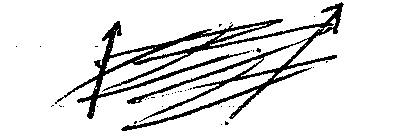
\includegraphics[width=\linewidth]{figures/gelfand-0152-p001398-cancelled-sketch-original-r2.png}\par\smallskip
{\footnotesize Original manuscript detail: \texttt{GELFAND-P001398}}
\end{minipage}\hfill
\begin{minipage}[t]{.50\linewidth}\vspace{0pt}\centering
{\footnotesize Partial visible-stroke recreation}\par\smallskip
% Visible pointed strokes and cancellation only; no node labels are recovered.
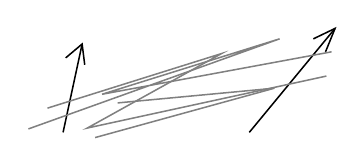
\begin{tikzpicture}[x=1.10cm,y=1.10cm,line width=.55pt]
\draw (0,0)--(.22,1.02);
\draw (.03,.86)--(.22,1.02)--(.25,.78);
\draw (2.15,0)--(3.14,1.20);
\draw (2.89,1.08)--(3.14,1.20)--(3.03,.93);
\draw[gray] (-.40,.04)--(2.50,1.08)--(.45,.44)--(3.1,.93);
\draw[gray] (-.18,.28)--(1.83,.91)--(.28,.05)--(3.04,.65);
\draw[gray] (.37,-.06)--(2.44,.51)--(.63,.34);
\end{tikzpicture}

\end{minipage}
\end{center}
\noindent{\small\textit{Only the visible pointed strokes and cancellation are recreated. No hidden node letters, arrow labels or connections are supplied.}}


\underline{\underline{Definition 2}}. An exact triangle in $K(A)$ or $D(A)$ is
a triangle isomorphic to the triangle:
\begin{center}
\begin{tikzcd}[column sep=small]
{} \arrow[r] & X \arrow[r,"f"] & Y \arrow[r,"g"] & C(f) \arrow[r] &
X[1] \arrow[r] & Y[1] \arrow[r] & \cdots
\end{tikzcd}
\end{center}


\EnglishSourceFrame{GELFAND-P001399}{unlabelled}
\underline{9/XI-87.}\qquad \underline{\underline{Gelfand seminar}}

[Crossed out: Lascoux.]\qquad \underline{Lascoux}

\underline{I. M. G. following Lascoux}
(\EnglishUnclear{GELFAND-P001399}{heading-parenthesis}{beautiful / correct} series)

Schubert polynomials.

Consider the polynomial
\begin{equation*}
P=\alpha u+\beta\EnglishUnclear{GELFAND-P001399}{equation-1-second-variable}{u\text{ or }v}+\gamma w+\cdots \tag{1}
\end{equation*}
$u,v,w$ [crossed out: \EnglishUnclear{GELFAND-P001399}{cancelled-coefficients}{$\alpha,\beta,\gamma$}] are monomials.

In our case, we will have $u,v,w,$ [one sign crossed out:
\EnglishUnclear{GELFAND-P001399}{cancelled-after-w}{illegible}] $\ldots=x_1,x_2,\ldots,x_n$.

$\alpha,\beta,\gamma,\ldots$ are numbers.

The polynomials [crossed out: \EnglishUnclear{GELFAND-P001399}{cancelled-before-sm}{function / functions [source abbreviations]}]
$S^m(P)$ [crossed out: \EnglishUnclear{GELFAND-P001399}{cancelled-after-sm}{Schur}]
are defined by the formula
\begin{equation*}
\sum_{\EnglishUnclear{GELFAND-P001399}{equation-2-lower-bound}{m\ge0\text{ or }m=0}}^{\infty}
z^m S^m(P)=\frac{1}{(1-zu)^\alpha(1-zv)^\beta\ldots} \tag{2}
\end{equation*}
\begin{equation*}
\alpha=\beta=\gamma=\cdots=1\quad\Rightarrow
\end{equation*}
\begin{equation*}
S^m(x_1+x_2+\cdots+x_n)=\sum_{i_1\le i_2\le\cdots\le i_m}
x_{i_1}x_{i_2}\cdots x_{i_m} \tag{3}
\end{equation*}

For example,
\begin{equation*}
S^2(x_1+x_2)=x_1^2+x_1x_2+x_2^2
\end{equation*}

Consider the Hankel matrix (of infinite order):
\begin{equation*}
\begin{pmatrix}
S^0(P)&S^1(P)&S^2(P)&\ldots\\
S^{-1}(P)&S^0(P)&S^{\EnglishUnclear{GELFAND-P001399}{matrix-row-2-col-3}{4\text{ or }1}}(P)&\ldots\\
&&&
\end{pmatrix},\qquad S^{-i}(P)=0\text{ for }i>0. \tag{4}
\end{equation*}

(See \underline{Akhiezer}'s book on the moment problem.)

Multiplication of the series (2) corresponds to multiplication of the matrices (4).


\EnglishSourceFrame{GELFAND-P001400}{30}
\underline{A topic in operator theory which I. M. G. proposed to
\EnglishUnclear{GELFAND-P001400}{heading-recipient}{Birman / Burman}:}

\EnglishUnclear{GELFAND-P001400}{heading-verb}{Connect / Connection / Make}
the $K$-functor in operator theory

(Fifteen years later, Sato had already done this.)

And it became fashionable.

\underline{The only theorem from matrix theory}

Consider the matrix $A$: $f_{\alpha\beta}=f(\alpha,\beta)$ and all of its minors
of order $k$: these also form a matrix (the compound matrix of order $k$),
$\Lambda^k(A)$. Then
\begin{equation*}
\Lambda^k(AB)=\Lambda^k(A)\Lambda^k(B) \tag{5}
\end{equation*}

It is convenient to denote the row numbers by $i_1+1,i_2+2,\ldots,i_p+p$ and the column numbers by
$j_1+1,j_2+2,\ldots,j_p+p$:
\begin{equation*}
\left|\begin{aligned}
i_1&\le i_2\le\cdots\le i_p\\
j_1&\le\cdots\le j_p
\end{aligned}\right.
\end{equation*}

\begin{equation*}
S_{J\mid I}(P)\quad\text{--- the corresponding minor, called a }\underline{\text{skew Schur function}}. \tag{6}
\end{equation*}
\begin{equation*}
S_{J\mid 0}(P)\quad\text{--- an ordinary Schur function.}
\end{equation*}

[Crossed out: Then] One can consider the polynomial (Jacobi)
\begin{equation*}
\frac{
\begin{vmatrix}
x_1^{j_1}&x_1^{j_2+1}&\ldots&x_1^{j_p+p-1}\\
x_2^{j_1}&x_2^{j_2+1}&\ldots&x_2^{j_p+p-1}\\
\ldots&\ldots&\ldots&\ldots
\end{vmatrix}
}{
\begin{vmatrix}
1&x_1&\ldots&x_1^{p-1}\\
1&x_2&\ldots&x_2^{p-1}\\
&&&\\
1&x_p&\ldots&x_p^{p-1}
\end{vmatrix}
} \tag{7}
\end{equation*}
[In the first two rows of the numerator, after $j_1$, crossed out:
\EnglishUnclear{GELFAND-P001400}{numerator-first-column-cancellations}{$+1$ / $+0$}.]

[To the right of the numerator: \EnglishUnclear{GELFAND-P001400}{right-of-numerator}{1 / a single slanting stroke}.]

(\EnglishUnclear{GELFAND-P001400}{exercise-number}{8 / 7})
([Inserted above the line: \underline{Exercise}] Check that the numerator is divisible by the denominator!)

[Crossed out: \EnglishUnclear{GELFAND-P001400}{cancelled-before-eto}{ko / but [source candidates: «ко» / «но»]}.]
This is a symmetric function, but its coefficients are not explicitly
[crossed out: \EnglishIncomplete{GELFAND-P001400}{cancelled-right-word}{The cancelled word beneath the inserted ``written'' has not been read.}]
[inserted above the line: \underline{written}]
and are still being studied.

[In the left margin: (\EnglishUnclear{GELFAND-P001400}{margin-first-line}{first steps / new steps}
\EnglishIncomplete{GELFAND-P001400}{margin-second-line}{The second line of the small addition before the bibliographical reference has not been read.})]

(See the paper by [crossed-out initials:
\EnglishUnclear{GELFAND-P001400}{bibliography-cancelled-initials}{I. G. / I. M.};
inserted above them: \underline{I. M.}] Gelfand, Zelevinsky, 1986, FA;
and the unpublished work of B. \EnglishUnclear{GELFAND-P001400}{bibliography-last-name}{Lidsky / Litsky}.)

\underline{It is clear} \EnglishUnclear{GELFAND-P001400}{penultimate-word}{so far / only} that the coefficients
[crossed out: \EnglishUnclear{GELFAND-P001400}{cancelled-before-integers}{all / will be}] are integers.

Schur realised that they are important:
\EnglishUnclear{GELFAND-P001400}{last-line-verb}{commented on / having commented on}
Jacobi, Frobenius and others.


\EnglishSourceFrame{GELFAND-P001401}{unlabelled}

Frobenius found the characters of the symmetric group; this is profound work which
is not replaced by H. Weyl's comments.

(9) \underline{Theorem.} (Jacobi--Trudi)

\begin{equation*}
(10)\qquad (7)=S_{J/0}(x_1+\ldots+x_p)
\end{equation*}

(11) \underline{Problem:} a) \EnglishUnclear{GELFAND-P001401}{task-a}{bring down [source candidate: osadit'] / comprehend};

b) give its classical proof;

c) give an interpretation in representation theory.

(12) $S_{J/I}$ satisfies a system of identities;
these are Pl\"ucker coordinates (one of Sato's achievements!).

\begin{equation*}
(13)\qquad
S^{\text{\EnglishUnclear{GELFAND-P001401}{formula-13-power}{n / m}}}(P+Q)
=\sum_j S^{n-j}(P)S^j(Q);
\end{equation*}

\begin{equation*}
(14)\qquad
S^n(PQ)=\sum_{|J|=n}S_J(P)S_J(Q),\qquad S_J=S_{J/0};
\end{equation*}

\begin{equation*}
(15)\qquad
S^n(S^m(P))=\sum(n,m;J)S_J(P)
\quad\text{\EnglishUnclear{GELFAND-P001401}{formula-15-end}{$\Vert$ / a crossed-out sign}},
\end{equation*}

where $(n,m;J)$ are universal coefficients.

The cohomology of flag manifolds is calculated in two ways:

a) decomposition into Schubert cells (the dimensions are even!);

b) differential forms.

Which forms correspond to which cells?

Schubert polynomials arise here

(up to symmetric ones).

\underline{Lascoux, Sch\"utzenberger:} one must forget topology and calculate polynomials.

The polynomials must be \EnglishUnclear{GELFAND-P001401}{last-line-word}{settled [source candidate: poselit']}
in the ring of all polynomials, and so on.


\EnglishSourceFrame{GELFAND-P001402}{31}

[The following fragment is circled and crossed out:]

(16) \underline{Theorem.} Permute the rows
\begin{equation*}
h_1+1,\ h_2+2,\ldots,h_p+p,\qquad h_1\le h_2\le\ldots\le h_p;
\end{equation*}

Newton introduced the operations

\begin{equation*}
(16)\qquad
\partial_i f(x_1,\ldots,x_n)=
\frac{f(x_1,\ldots,x_{i+1},x_i,\ldots,x_n)-f(x_1,\ldots,x_i,x_{i+1},\ldots,x_n)}{x_{i+1}-x_i}
\end{equation*}

Then

\begin{equation*}
(17)\qquad
\left\{
\begin{aligned}
&\partial_i^2=0\\
&\partial_i\partial_j=\partial_j\partial_i,\qquad |i-j|\ge2,\\
&\partial_i\partial_{i+1}\partial_i=\partial_{i+1}\partial_i\partial_{i+1}
\end{aligned}
\right.
\end{equation*}

(18) \underline{Remark.}
\begin{equation*}
(\partial_i+1)(\partial_i-q)=0
\quad\Rightarrow\quad
\partial_i\text{ --- a $q$-analogue of the generators of the symmetric group}
\end{equation*}
\begin{equation*}
q=1\quad\Rightarrow\quad\text{the symmetric group}
\end{equation*}

(instead of $(17)_{\text{\EnglishUnclear{GELFAND-P001402}{remark-18-subscript}{1 / a}}}$)

\underline{\underline{Lascoux}}

\underline{The relation between Schubert polynomials and Schur functions.}

(19) $\partial_i(fg)=g\partial_i(f)$ if
[crossed out: \EnglishUnclear{GELFAND-P001402}{cancelled-19-symbol}{$f$}]
$g$ is symmetric with respect to the
[crossed out: \EnglishIncomplete{GELFAND-P001402}{cancelled-19-word}{The word is covered by several strokes; ``all'' / ``two'' are possible, but the whole word has not been established.}]
variables $x_i,x_{i+1}$.

A reminder about Schubert polynomials:
\begin{equation*}
Y_{730}=x_1^7x_2^3x_3^0
\end{equation*}

(20) \underline{Definition.} If $\underbrace{i_1\ge i_2\ge i_3\ge\ldots}_{I}$, then
$x_1^{i_1}x_2^{i_2}\ldots=Y_I$.

(The Schubert polynomial
[crossed out: \EnglishUnclear{GELFAND-P001402}{note-20-first-sign}{$I$ / $=$}]
[crossed out: \EnglishIncomplete{GELFAND-P001402}{note-20-cancelled-word}{A short entry is covered by horizontal strokes; complete letters and the word cannot be recovered from the scan.}]
with index $I$ is a monomial.)

All Schubert polynomials \EnglishUnclear{GELFAND-P001402}{all-schubert-sign}{$=$}
are images of these under arbitrary combinations of $\partial_i$.

[Above the word ``images'', inserted: ``(all nonzero ones)''.]

\underline{Rule for \EnglishUnclear{GELFAND-P001402}{rule-abbreviation}{rasch. / rab. [unexpanded source abbreviations]} indices}

\begin{equation*}
(21)\qquad
Y_{\ldots i_p i_{p+1}\ldots}
\overset{\partial_p}{\longrightarrow}
\begin{cases}
Y_{\ldots i_{p+1}\,i_p-1},&i_p>i_{p+1}\\
0,&\text{otherwise}
\end{cases}
\end{equation*}

\underline{Exercise:} Prove that these definitions are well-defined.

(22) \underline{Example}
\begin{equation*}
Y_{730}=x_1^7x_2^3x_3^0=
\begin{vmatrix}
S^3(x_1+x_2)&S^8(x_1)\\
S^2(x_1+x_2)&S^7(x_1)
\end{vmatrix}
\end{equation*}


\EnglishSourceFrame{GELFAND-P001403}{unlabelled}

(23)

[In the first line, after the fraction and before the equals sign, crossed out:
\EnglishIncomplete{GELFAND-P001403}{generating-cancelled}{A short entry is crossed by a horizontal line; the visible lower curves and right stroke do not establish its text or formula.}]

\begin{equation*}
\begin{tikzcd}[column sep=small,row sep=large]
{\displaystyle\frac{1}{(1-zx_1)(1-zx_2)}}\arrow[d,"\partial_2"]
& {=\displaystyle\sum z^j S^j(x_1+x_2)}\\
{\displaystyle\frac{z}{(1-zx_1)(1-zx_2)(1-zx_3)}} &
\end{tikzcd}
\end{equation*}

\begin{equation*}
(23)\qquad
S^n(x_1+x_2)\overset{\partial_2}{\longrightarrow}
S^{n-1}(x_1+x_2+x_3)
\end{equation*}

From (22), we obtain

(24)
\begin{equation*}
\begin{tikzcd}[column sep=small,row sep=large]
{\partial_2Y_{730}}
& {=\begin{vmatrix}S^2(x_1+x_2+x_3)&S^8(x_1)\\S^1(x_1+x_2+x_3)&S^7(x_1)\end{vmatrix}}
& {=Y_{702}}\arrow[d,"\partial_1"]\\
& {\begin{vmatrix}S^2(x_1+x_2+x_3)&S^7(x_1+x_2)\\S^1(x_1+x_2+x_3)&S^6(x_1+x_2)\end{vmatrix}}\arrow[d,"\partial_2"]
& {=Y_{062}}\\
{Y_{025}}\arrow[d,equal]
& {=\begin{vmatrix}S^2(x_1+x_2+x_3)&S^6(x_1+x_2+x_3)\\S^1(x_1+x_2+x_3)&S^5(x_1+x_2+x_3)\end{vmatrix}}
&\\
{S_{025}(x_1+x_2+x_3)}&&
\end{tikzcd}
\end{equation*}

(The Schur function defined earlier; $S_{025/0}(x_1+x_2+x_3)$;
families of zeros are omitted.)

Writing formula
[crossed out: \EnglishIncomplete{GELFAND-P001403}{bottom-cancelled-word}{The word is covered by several intersecting strokes; the conjecture ``Schur'' is not fully confirmed by the visible letters.}]
(22) as a determinant was used
in elimination theory in the nineteenth century.

\underline{There are five (thick) volumes of the book}

\underline{T. Muir}: History of Determinants, Dover (1960)


\EnglishSourceFrame{GELFAND-P001404}{32}

There is also a book (by the same author):

Theory of determinants

(\EnglishUnclear{GELFAND-P001404}{book-parenthesis}{only formulas / thousands of formulas})

(one volume)

\underline{500 pages}

[To the right of the title, two entries separated by a vertical line:]
everything before \fbox{1900} $\vert$ almost everything before (1920)

[An arrow downwards from the book title:] available at IPM [source abbreviation].

\underline{Analogy}: the theory of integrable systems, \EnglishUnclear{GELFAND-P001404}{analogy-verb}{construct [perfective] / contains / construct [imperfective]} a theory for these formulas.

(25) \underline{Theorem.}
\EnglishUnclear{GELFAND-P001404}{theorem25-left-index}{$S_{I\mid000}$ / $S_{I1000}$}
$(x_1+\dots+x_n)=Y_{i_1\dots i_n0000}$

$0\leq i_1\leq\dots\leq i_n$

(26) Finite case:
\EnglishUnclear{GELFAND-P001404}{finite26-left}{$\mathbb{Z}[x_1,x_2,\dots,x_n]$ / $\mathbb{Z}[x_1,x_2,\dots,x_{n+1}]$}
$\big/$ideal of symmetric polynomials in
$(x_1,x_2,$
[crossed out: \EnglishUnclear{GELFAND-P001404}{finite26-cancelled}{$x_3$? / $x_n$?}]
$\dots,x_{n+1})$

(27) \underline{Theorem.} The Schubert polynomials

(28)
\begin{equation*}
Y_I,\quad 0\leq i_1\leq n,\quad
0\leq i_2\leq n-1,\quad\dots,\quad
0\leq i_{n+1}\leq0
\end{equation*}
form a basis of the ring (26) as a free abelian group.

\underline{Example}

$\underline{n=2}\qquad\mathfrak{S}(3);$
\begin{equation*}
Y_{210}\qquad Y_{110}\qquad Y_{200}\qquad
Y_{010}\qquad Y_{100}\qquad Y_{000}
\end{equation*}
A $\mathbb{Z}$-basis of $\mathbb{Z}[x_1,x_2,x_3]/(\qquad)$

It follows from (27) that the dimension is
\EnglishUnclear{GELFAND-P001404}{dimension-factorial}{$n!$ [as in the source]}.

The others fall into the ideal:

(29)
\begin{equation*}
Y_I\in\mathrm{ideal}\qquad\text{if}\qquad I\leq\!\!\!/\,210
\end{equation*}

(30) \underline{Question from I. M. G.}: how is the representation of $\mathfrak{S}(n)$ written
[crossed out: \EnglishUnclear{GELFAND-P001404}{question30-cancelled}{in? / an illegible sign}]
when $\mathfrak{S}(n)$ acts on the variables $x_1,\dots,x_n$ in Schubert
polynomials?

In the cohomology ring
[inserted above the line, with an insertion mark:
(\EnglishUnclear{GELFAND-P001404}{cohomology-insertion}{mn-iya / mn-giya [unexpanded source abbreviations]} of flags)]
there is a quadratic form written as follows:

(31)
\begin{equation*}
PQ\overset{\partial_1\partial_2\partial_1}{\longrightarrow}(P,Q)
\end{equation*}
(inner product)

[On the right:] (a number in the quotient by the ideal)

(32) \underline{Chevalley theorem.}

$\partial_1$ is symmetric with respect to $(\ ,\ )$.

$\partial_2$ --- '' --- [repetition mark]

[On the left:] s.u. [unexpanded source abbreviation: «с.у.»]

(33)
\begin{equation*}
(\partial_1(P),Q)=(P,\partial_1(Q))
\end{equation*}

The proof is not difficult.

Lascoux.

(34)
\begin{equation*}
Y_I,\qquad Y_{I'},\qquad I+I'=n\quad n-1\quad\dots\quad1\quad0
\end{equation*}

